%!TEX program = xelatex
%!TEX encoding = UTF-8 Unicode

\documentclass[14pt, AutoFakeBold]{ldr}
  

\title{本 科 生 毕 业 答 辩}
\subtitle{利用机器学习进行气体探测器径迹重建的算法研究}

\author{答辩人:王文军}
\institute{指导老师:张毅}
\date{\today}
\titlegraphic{
\includegraphics[height=0.15\textwidth]{lzu_logo.png}}



  



\begin{document}

\maketitle

\AtBeginSection[]
{
  \begin{frame}
    \frametitle{\insertshorttitle}
    \tableofcontents[currentsection,hideallsubsections]
  \end{frame}
}





\section{研究背景}
\subsection{基于裂变时间投影室的新型核裂变测量技术}
\begin{frame}[c]{基于裂变时间投影室的新型核裂变测量技术}
利用机器学习进行\textcolor{red}{气体探测器径迹重建}的算法研究


  \frametitle{基于裂变时间投影室的新型核裂变测量技术}
  \begin{figure}[H]
  \centering
  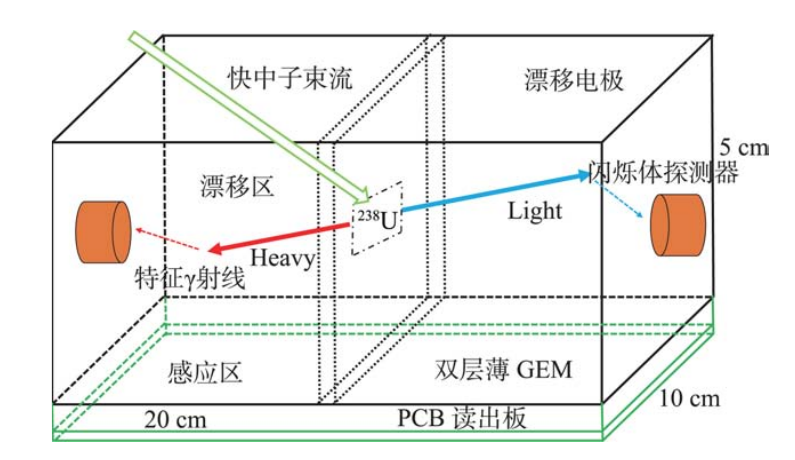
\includegraphics[width=0.9\textwidth]{../figures/GEM-TPC.png}

  \caption{裂变时间投影室探测系统(论文 P6)}
  \label{fig-GEM-TPC}
  \end{figure}
  
\end{frame}



\begin{frame}
  \frametitle{时间投影室的应用}
  \begin{itemize}
    \item 许多大型高能粒子实验都采用其作为中心径迹探测器, 比较著名的有LEP实验的ALEPH, DELPHI, BNL的 STAR, LHC的ALICE等等。
    \item MicroBooNE Collaboration 应用卷积神经网络完成了对时间投影室产生的径迹数据的算法研究。算法包括多粒子径迹图片的分类(Classification)、多粒子径迹图片中的空间定位(Localization)。
    \end{itemize}
\end{frame}



\begin{frame}
  \frametitle{时间投影室的目前的局限}
  \begin{itemize}
    \item 对于裂变碎片的鉴别尚处于空白。
    \item 对于裂变碎片的径迹重建仍然基于经典的离子能损理论。
    \item 如果将径迹简单地拟合为直线无法准确处理这种非线性效应。
    \end{itemize}
    
    \begin{figure}[H]
      \centering
      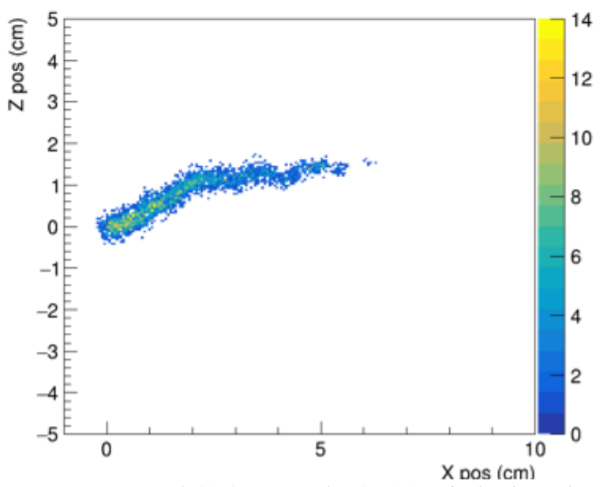
\includegraphics[width=0.5\textwidth]{../figures/Snipaste_2021-05-20_16-39-55.png}
    
      \caption{模拟的裂变碎片径迹在读出板上的信号}
      \label{fig-Test}
  \end{figure}
\end{frame}



\begin{frame}[t]
  \frametitle{深度学习人工神经网络的优点}
  利用\textcolor{red}{机器学习}进行气体探测器径迹重建的算法研究

  $\linebreak$
  $\linebreak$

  深度学习人工神经网络的优点:
  \begin{itemize}
    \item 能够近似模拟任何数学函数。
    \item 人工神经网络对非线性数据具有最好的甄别效果。
    \item 易于实现。
    \end{itemize}

\end{frame}




\section{基于裂变时间投影室的径迹重建}
\begin{frame}[c]
  \frametitle{径迹重建流程}

  \begin{figure}[H]
    \centering
    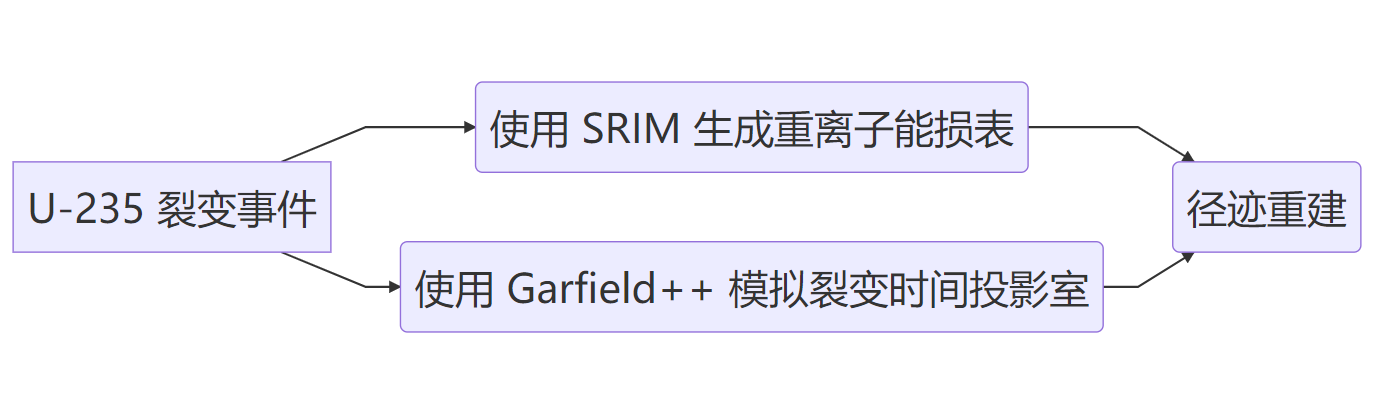
\includegraphics[width=1.0\textwidth]{../figures/flowchart.png}
    \caption{径迹重建流程}
    \label{fig-flowchart1}
    \end{figure}

    
\end{frame}


\begin{frame}[c]
  \frametitle{二维径迹图像}
    \begin{figure}[H]
      \centering
      \subfloat[37N95]{
            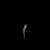
\includegraphics[width=0.3\textwidth]{../figures/0.00236_-0.4095_0.91231.out_all_electrodes_double.png}
        }
      \subfloat[37N95]{
            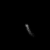
\includegraphics[width=0.3\textwidth]{../figures/0.571_0.48881_0.65957.out_all_electrodes_double.png}
        }
      \subfloat[37N95]{
            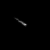
\includegraphics[width=0.3\textwidth]{../figures/-0.7673_-0.39935_-0.50177.out_all_electrodes_double.png}
        }\\	
        \caption{二维径迹图}
        \label{fig_track_2d_2}
    \end{figure}
\end{frame}





\section{基于人工神经网络的裂变碎片分类模型}
\begin{frame}[c]
  \frametitle{使用 fastai 搭建人工神经网络}

  \begin{figure}[H]
    \centering
    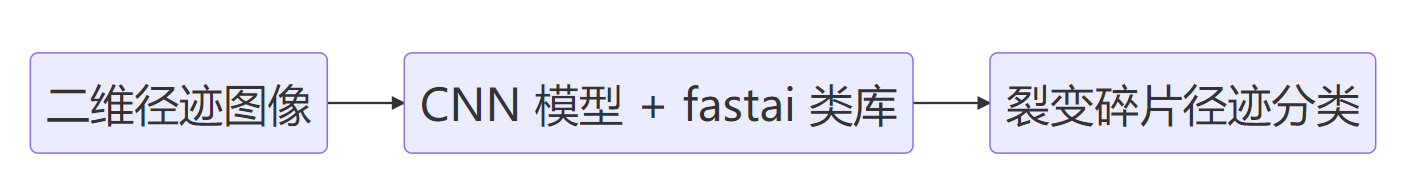
\includegraphics[width=1.0\textwidth]{../figures/flowchart3.png}
    \caption{神经网络模型建立流程}
    \label{fig-flowchart3}
    \end{figure}
  
    CNN (Convolutional Neural Network, 卷积神经网络) 模型:ResNet, XResNet, DenseNet, VGG, SqueezeNet, ShuffleNet
\end{frame}



\begin{frame}[c]
  \frametitle{训练结果}
  目前最好可以同时对 6 种核素(39N100, 53N136, 37N95, 55N141, 40N102, 52N134)以不低于 99.5\% 的正确率完成分类。
  \begin{figure}[H]
    \centering
    \subfloat[Accuray]{
          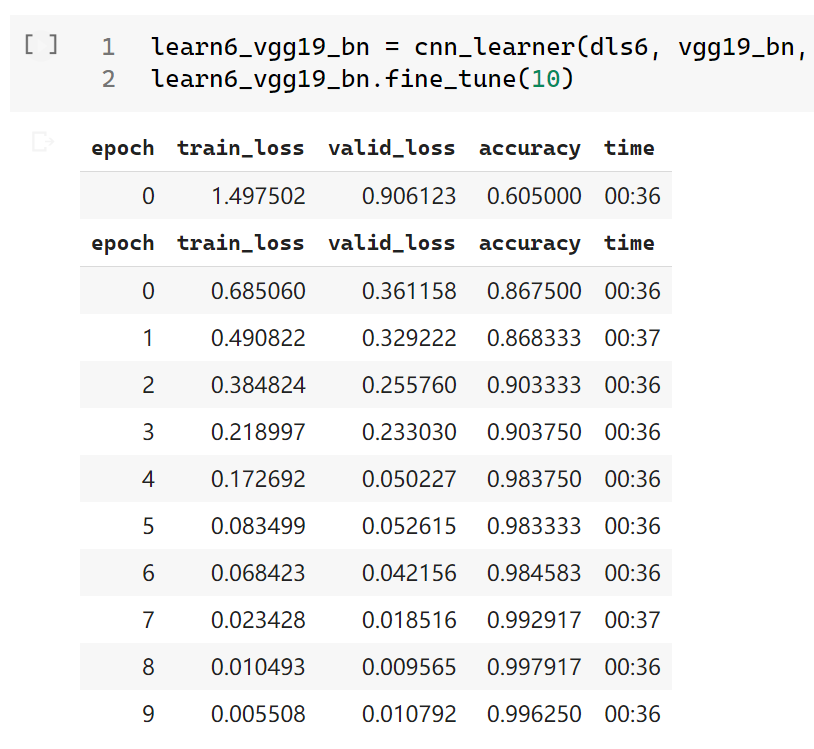
\includegraphics[width=0.4\textwidth]{../figures/learn6-vgg19-bn.png}
      }
    \subfloat[Loss]{
          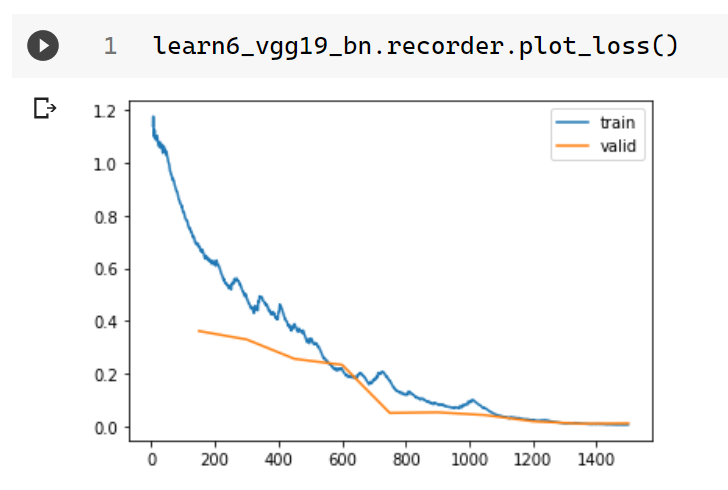
\includegraphics[width=0.4\textwidth]{../figures/learn6-vgg19-bn-loss.png}
      }\\	
      \caption{6 种核素训练结果(VGG19\_bn)}
      \label{fig_learn6_vgg19-bn}
  \end{figure}
  
\end{frame}


\begin{frame}[c]
  \frametitle{网络测试}

  \begin{figure}[H]
    \centering
    \subfloat[37]{
          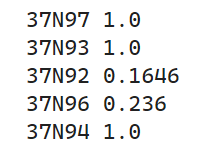
\includegraphics[width=0.2\textwidth]{../figures/37-result.png}
      }
      \subfloat[39]{
          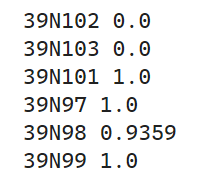
\includegraphics[width=0.2\textwidth]{../figures/39-result.png}
      }
    \subfloat[40]{
          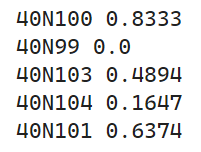
\includegraphics[width=0.2\textwidth]{../figures/40-result.png}
      }\\	
      \subfloat[52]{
          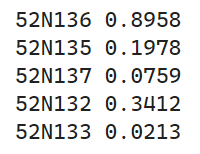
\includegraphics[width=0.2\textwidth]{../figures/52-result.png}
      }
      \subfloat[53]{
          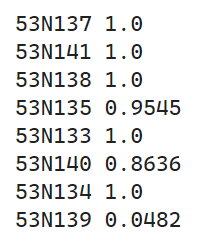
\includegraphics[width=0.2\textwidth]{../figures/53-result.png}
      }
    \subfloat[55]{
          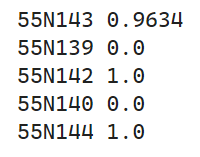
\includegraphics[width=0.2\textwidth]{../figures/55-result.png}
      }\\	
      \caption{测试结果}
      \label{fig-test-output}
  \end{figure}
  
\end{frame}



\section{总结展望}

\begin{frame}[c]
  \frametitle{总结}
  本论文从模拟计算产生的 $^{235}$U 裂变碎片事件数据出发,使用 SRIM 生成每一个核素的重离子能损表,然后使用 Garfield++ 调用 SRIM 的重离子能损表估算每一个裂变碎片在时间投影室内的径迹信息,完成裂变碎片的在时间投影室内的二维重建和三维径迹重建。

  $\linebreak$

之后使用 fastai,以二维径迹图像为输入数据,完成了裂变碎片径迹图像的鉴别分类。建立的网络模型最好可以同时对 6 种核素以不低于 99.5\% 的准确率完成核素分类,除此之还,还可以对 12 种核素以不低于 80\% 的正确率完成分类。
  
\end{frame}


\begin{frame}[c]
  \frametitle{展望}
  \begin{itemize}
    \item 增大数据量(单个核素径迹数、总核素数目)
    \item 提高径迹数据精度
    \item 将粒子的能损(dE/dx)信息加入输入层
    \end{itemize}
  
\end{frame}



\end{document}